
%---------------------------------------------------------------------
% CAPA
%---------------------------------------------------------------------

\renewcommand{\imprimircapa}{%
	\begin{capa}%
		\center
		\begin{tikzpicture}[remember picture,overlay] 
			\node[anchor=south west, yshift= 25mm, xshift=-1.5mm] at 
			(current page.south west) 
			{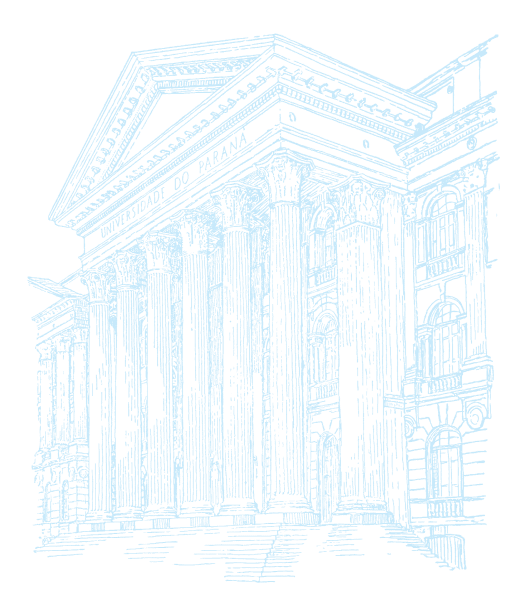
\includegraphics[width = \paperwidth]{Imagens/capa_UFPR}};
		\end{tikzpicture}
		\center
		%    \ABNTEXchapterfont 
		\MakeUppercase\imprimirinstituicao \vspace{-2mm}
		
		%\ifthenelse{\equal \ImprimirSetor{}}{}{
			%    \ABNTEXchapterfont 
		%	\MakeUppercase\ImprimirSetor}
		%\vspace{-2mm}
		
		%\ifthenelse{\equal \ImprimirProgramaPos{}}{}{
		%	     \ABNTEXchapterfont 
		%	\MakeUppercase\ImprimirProgramaPos}
		
		\ifthenelse{\equal \ImprimirCurso{}}{}{
			%    \ABNTEXchapterfont 
			\MakeUppercase\ImprimirCurso}
		
		\vspace{40mm}
		
		%    \ABNTEXchapterfont 
		\MakeUppercase\imprimirautor
		
		\vspace{40mm}
		%    \ABNTEXchapterfont
		\MakeUppercase\imprimirtitulo
		\vfill
		
		%\large
		\MakeUppercase\imprimirlocal
		
		%\large
		\imprimirdata
		
		\vspace*{10mm}
	\end{capa}
}

\pdfbookmark[0]{Capa}{Capa}
\imprimircapa


